%%
%% Template chap1.tex
%%

\chapter{Background}
\label{cha:background}

\section{First-Order Logic Terms and Notation}
\label{sec:fol}

This thesis focuses around the extension of \beagle, a \emph{first-order logic} (FOL) theorem prover.
In order to understand beagle's purpose and functions a basic understanding of the FOL logical system
is required. This section provides a rudimentary overview of FOL syntax and uses;
but also includes an explanation of any specialised terms and notation used throughout the paper.

\subsection{FOL basics}
\notes{
Should contain
\begin{itemize}
\item Variables
\item Symbols
\item Predicates
\item Quantifiers
\item Notion of soundness and completeness
\item Description of a 'calculus'
\end{itemize}}

\subsection{FOL with Equality and Ordering}

\subsection{Important Terminology}
\label{sec:terminology}

\subsubsection{Positions}
Many concepts in this paper require the ability to precisely point out a specific
subterm/symbol within a term. Thus we introduce a syntax for term \emph{positions}.
This sort of syntax is a standard concept in the field of logic; but here we
will be using a slightly extended syntax as we will have need to reference
positions which do not exist \cite{shulz12}.

A \emph{position} is given as a (possibly empty) list of natural numbers.
$t|_p$ refers to the subterm of $t$ at position $p$.
The empty position, $t|_\epsilon$, refers to the outermost function or variable
of a term. A position $t|_n$ refers to the $n^{th}$ argument of the outermost function,
$t|_{n.m}$ to the $m^{th}$ argument of that $n^{th}$ argument; and so on. If the position
does not exist in the term we return Nil. Consider the following example:
\[t = f(a, g(a, x, y), b)\]
\[t|_{\epsilon} = f \quad\quad t|_{1} = a \quad\quad  t|_{2.2} = x \quad\quad  t|_{2.3.3} = \text{Nil} \quad\quad  t|_{3.2} = \text{Nil}\]

\subsubsection{Substitution}

\subsubsection{Subsumption}

\subsubsection{Unification}

%\subsection{Popular Problems in First Order Logic}

\subsection{The Superposition Calculus}
\label{sec:supcalc}

\cite{supcalc} \cite{smartmatch}

\begin{align*}
\textbf{Positive Superposition} &&& \frac{l \approx r \lor C\quad \quad s[u] \approx t \lor D}{(s[r] \approx t \lor C \lor D)\sigma}
\intertext{\tcent{Where $\sigma = $ mgu $(l,u)$, and $u$ is not a variable}}
\textbf{Negative Superposition} &&& \frac{l \approx r \lor C\quad \quad s[u] \not\approx t \lor D}{(s[r] \not\approx t \lor C \lor D)\sigma}
\intertext{\tcent{Where $\sigma = $ mgu $(l,u)$, and $u$ is not a variable}}
\textbf{Equality Resolution}    &&& \frac{s \not\approx t \lor C}{C\sigma}
\intertext{\tcent{Where $\sigma = $ mgu $(s,t)$}}
\textbf{Equality Factoring}     &&& \frac{l \approx r \lor s \approx t \lor C}{(l \approx t \lor r \not \approx t \lor C)\sigma}
\intertext{\tcent{Where $\sigma = $ mgu $(s,l)$}}
\end{align*}


\section{Automated Reasoning and Theorem Proving}
\label{sec:proving}

Automated Reasoning is a rapidly growing field of research where computer programs
are used to solve formal logic problems; typically stated in first-order logic.

Some existing resolution theorem provers include:

\subsection{SPASS}
\cite{spass}

\subsection{Vampire}
\cite{vampire}

\subsection{E}
\cite{eprover}

\section{Term Indexing}
\label{sec:indexing}


Term indexing is a technique used to better locate clauses and terms for which inference rules
in a calculus will apply. In particular, indexers are used to find all terms which
will or are likely to \emph{unify} or \emph{match}; which is a typical condition
of any inference rule (for example all rules for the superposition calculus
in Section \ref{sec:supcalc} require some unifier $\sigma$).
The process of implementing Term Indexing forms the core of this paper. Our goal
is to implement a recent technique known as Fingerprint Indexing (see Section \ref{sec:fingerprint});
but for examples and comparison we present here some other techniques.
Refer to \cite{indexing} for more detailed specifications of these techniques along
with some results comparing them.

\subsubsection{Top Symbol Hashing}
Top symbol hashing simply compares the outermost symbol of any two terms and checks
that they are compatible. For example, for the term $f(a,x)$ it would simply look
at the symbol $f$ and present any other term with the top symbol $f$ (or a variable) as compatible.

Top symbol hashing is provided as a simple example; it is very rudimentary and
is certainly not in active use by any popular theorem provers.

\subsubsection{Discrimination Trees}

Discrimination Trees are a \emph{perfect} indexing technique in that anything
returned by the indexer is guaranteed to be unifiable in some way. This advantage
is offset by taking a considerable amount of to retrieve terms.

The technique works by storing terms in a tree at a position determined by the structure
of each term. Each branch in the tree has a label which is either a function symbol
(e.g. $f$, $g$) or *, which may represent any variable. To place a term in the tree
we traverse the term from left to right and follow or create branches according to
which symbol we observe. This process is simple. but retrieving from the index is a
complex process requiring a backtracking algorithm.

Discrimination Trees have another distinct disadvantage in that their tree data
structure can grow arbitrarily large depending on the size and variety of observed terms.

\subsubsection{Path Indexing}

Path Indexing is currently in active use in the Vampire theorem prover \cite{vampire}.

\section{Fingerprint Indexing}
\label{sec:fingerprint}

\emph{Fingerprint Indexing} is a recent technique developed by \citeN{shulz12}, the creator
of the E prover. It works by computing a \emph{fingerprint} for each logic term;
which can compared for unification or match compatibility. 
Unlike some of the example techniques above,
Fingerprint Indexing is \emph{non-perfect} in that compatible fingerprints will not
always imply that the associated terms successfully unify/match. The technique
makes up for this by being adjustable to arbitrary levels of precision; ranging between
what essentially amounts to Top-Symbol Hashing (See section \ref{sec:indexing})
to comprehensive, but slow to compute, term comparisons.

\subsection{Term Fingerprints}
\label{sec:fingerprints}

A term's \emph{fingerprint} is a list of \emph{fingerprint features} which
indicate what the term looks like at a given position. The 4 possible
fingerprint features are:
\begin{itemize}
\item \textbf{A}: the term has a variable at the position.
\item $f$ (any function or constant in the current system): This
feature indicates that $f$ is at the given position in the term.
\item \textbf{B}: the position does not exist in the term, but can be created
by expanding a variable via substitution.
\item \textbf{N}: the position does not exist and cannot be created.
\end{itemize}
Term fingerprints are computed with respect to a list of positions. We do this by simply
computing which feature exists at each position. We will now revisit the example from
the explanation of term positions (Section \label{sec:terminology}) to show
the computation of a fingerprint. In the example $\{f,g\}$ are functions, $\{a,b\}$ are
constants and $\{x,y\}$ are variables.
\[t = f(a, g(a, x, y), b)\]
\[\text{positions} = [\epsilon, 1, 2.2, 2.3.3, 3.2] \]
\[t|_{\epsilon} = f \quad\quad t|_{1} = a \quad\quad  t|_{2.2} = x \quad\quad  t|_{2.3.3} = \text{Nil} \quad\quad  t|_{3.2} = \text{Nil}\]
\[\fp(t, \text{positions}) = [f, a, \textbf{A}, \textbf{B}, \textbf{N}] \]

\subsection{The Fingerprint Index}
\label{sec:fpindex}

Once a term's fingerprint has been generated we use it to store the term in a tree-like
data structure known as the \emph{Fingerprint Index}. 
This data structure is very reminiscent of a Discrimination Tree (See section \ref{sec:indexing})
and works similarly. To add a term to the index we (starting from the root node) follow/create
branches labelled with the fingerprint features of the term's fingerprint. Once the fingerprint has run
out we store the term in a leaf set. This process subtly indicates the key difference
between the Fingerprint Index and a Discrimination Tree: since all term fingerprints
are the same length, the Index has a fixed depth.

\begin{figure}[H]
  \centering
  \includegraphics[page=7,width=0.9\textwidth,trim=5cm 14.3cm 4.8cm 4.5cm,clip]{resources/schulz}
  \caption
   {Example structure of a Fingerprint Index. Taken unmodified from \protect\cite[p7]{shulz12}.}
   \label{fig:fpindex}
\end{figure}

\subsection{Comparing Fingerprints and Retrieving}

\begin{table}[h]\begin{center}
  \caption{Fingerprint Feature compare table for Unification \protect\cite[p6]{shulz12}}
  \label{tab:unif}
  \begin{tabular}{| c || c | c | c | c | c |}
  \hline
           &  $f_1$      &  $f_2$      &  \textbf{A} &  \textbf{B} &  \textbf{N} \\ \hline \hline
  $f_1$    &  \compY &  \compN &  \compY &  \compY &  \compN \\ 
  $f_2$    &  \compN &  \compY &  \compY &  \compY &  \compN \\ 
\textbf{A} &  \compY &  \compY &  \compY &  \compY &  \compN \\
\textbf{B} &  \compY &  \compY &  \compY &  \compY &  \compY \\ 
\textbf{N} &  \compN &  \compN &  \compN &  \compY &  \compY \\ \hline
  \end{tabular}
\end{center}\end{table}

\begin{table}[h]\begin{center}
  \caption{Fingerprint Feature compare table for Matching \protect\cite[p6]{shulz12}}
  \label{tab:match}
  \begin{tabular}{| c || c | c | c | c | c |}
  \hline
           &  $f_1$      &  $f_2$      &  \textbf{A} &  \textbf{B} &  \textbf{N} \\ \hline \hline
  $f_1$    &  \compY &  \compN &  \compN &  \compN &  \compN \\ 
  $f_2$    &  \compN &  \compY &  \compN &  \compN &  \compN \\ 
\textbf{A} &  \compY &  \compY &  \compY &  \compN &  \compN \\
\textbf{B} &  \compY &  \compY &  \compY &  \compY &  \compY \\ 
\textbf{N} &  \compN &  \compN &  \compN &  \compN &  \compY \\ \hline
  \end{tabular}
\end{center}\end{table}

\subsection{Position Variants}

\subsection{Why Fingerprint Indexing?}

In Section \ref{sec:indexing} we described several other techniques for indexing
terms, and many more than these few exist. It is then a natural question to ask:
why has Fingerprint Indexing been chosen as the focus of this paper?

Primarily due to how configurable it is. Also interesting to observe success
of a new technique rather than implementing something old.

\section{The \Beagle\ Theorem Prover}
\label{sec:beagle}

{\Beagle} was developed by Peter Baumgartner et al. of NICTA. as a proof of concept,
with the intention of demonstrating the capabilities of the \emph{\HSWAC}. This
calculus allows the incorporation of prior knowledge via \emph{background reasoning} modules. \cite{baum13}
These modules act as a sort of `black box' which we can use to rapidly prove
facts about background terms; without the need to convert them to an equivalent first-order logic
formulation. As a simple example we will think of the background reasoning module
as implementing integer arithmetic, but in practice these modules can be used to
incorporate essentially any collection of knowledge.

\Beagle\ itself is a resolution theorem prover like the examples above (Section \ref{sec:proving})
which implements this background reasoning calculus. This section provides a brief
summary of the capabilities of \beagle\ and the \HSWAC. For a detailed specification
of the precise advantages of the calculus refer to \cite{baum13}.

\subsection{Hierarchic Reasoning}
\label{sec:hier}
The logical calculus behind {\beagle} is not the first occurrence of using a hierarchy for
logical reasoning. A calculus was developed by \citeN{bach94} to take advantage
of this technique. Note that Waldmann continued on to co-write the paper outlining
{\HSWA} \cite{baum13}.

The hierarchic reasoning system also involves an ordering on terms.

\subsection{Weak Abstraction}
In order to keep the \emph{foreground} and \emph{background} reasoning
systems segregated it is necessary to clearly split a clause into its foreground
and background parts. This is where the process of \emph{weak abstraction} comes in.

In logics with equality there is a general process known as \emph{abstraction},
where a subterm within a clause may be replaced by a fresh variable.
\[\textbf{Abstraction}\quad\quad \frac{C[t]}{t\not\approx X \lor C[X]}\]
%In more intuitive English terms, this process says \emph{"If $t$ is equal to $X$ then we may replace it for $X$"}.
In a hierarchical calculus abstraction can be used to introduce new abstraction variables to take the place
of any background subterms. \citeN{bach94} extended this form of derivation to what they called \emph{full-abstraction},
where abstraction is performed exhaustively until no literal contains both foreground
and background operators.

In their recent paper however, \citeN{baum13} discovered that the process 
of full abstraction can destroy completeness; and they then go on to propose a new
variety of abstraction which they refer to as \emph{weak} abstraction. 
In weak abstraction only \emph{maximal background subterms which are
neither domain elements nor variables} are abstracted. Domain elements refer
to constant values in the background reasoning system, like 1 or 2 in the case of
integer arithmetic. A maximal background subterm
is a background subterm not contained in any other background subterm. Abstracted terms are replaced
with abstraction variables in the case of pure background terms, or ordinary variables
in the case of impure background terms. See the paper itself for weak abstraction
examples and details of how this process affects completeness.

\subsection{Rule Based Inference System}
\label{sec:calc}

The base inference rules for the {\HSWAC} are essentially identical to the standard 
superposition calculus; except for the fact that they come with many additional
conditions to accommodate background reasoning. These conditions include respecting
clause orderings and disallowing the use of pure background terms.

The results of any inferences must also have weak abstraction performed on them. This
ensures that we only ever have weakly abstracted terms in our logical system. The
base inference rules follow, taken directly from Section 6 of the {\HSWA} paper \cite{baum13}.
See Section \ref{sec:supcalc} to compare these rules to the original
superposition calculus.

\begin{align*}
\textbf{Positive Superposition} &&& \frac{l \approx r \lor C\quad \quad s[u] \approx t \lor D}{\text{abstr}((s[r] \approx t \lor C \lor D)\sigma)} 
\intertext{\tcent{Where
(i) $\sigma = $ simple mgu $(l,u)$,
(ii) $u$ is not a variable,
(iii) $r\sigma \not\succeq l\sigma$,
(iv) $t\sigma \not\succeq s\sigma$,\\
(v) $l$ and $u$ are not pure background terms,
(vi) $(l \approx r)\sigma$ is strictly maximal in $(l \approx r \lor C)\sigma$, and
(vii) $(s \approx t)\sigma$ is strictly maximal in $(s \approx t \lor D)\sigma$ }}
\textbf{Negative Superposition} &&& \frac{l \approx r \lor C\quad \quad s[u] \not\approx t \lor D}{\text{abstr}((s[r] \not\approx t \lor C \lor D)\sigma)}
\intertext{\tcent{Where 
(i) $\sigma = $ simple mgu $(l,u)$,
(ii) $u$ is not a variable,
(iii) $r\sigma \not\succeq l\sigma$,
(iv) $t\sigma \not\succeq s\sigma$,\\
(v) $l$ and $u$ are not pure background terms,
(vi) $(l \approx r)\sigma$ is strictly maximal in $(l \approx r \lor C)\sigma$, and
(vii) $(s \not\approx t)\sigma$ is strictly maximal in $(s \not\approx t \lor D)\sigma$ }}
\textbf{Equality Resolution}    &&& \frac{s \not\approx t \lor C}{\text{abstr}(C\sigma)}
\intertext{\tcent{Where 
(i) $\sigma = $ simple mgu $(s,t)$,
(ii) $s$ and $t$ are not pure background terms,\\ and
(iii) $(s \not\approx t)\sigma$ is strictly maximal in $(s \not\approx t \lor C)\sigma$}}
\textbf{Equality Factoring}     &&& \frac{l \approx r \lor s \approx t \lor C}{\text{abstr}((l \approx t \lor r \not \approx t \lor C)\sigma)}
\intertext{\tcent{Where 
(i) $\sigma = $ simple mgu $(l,u)$,
(ii) $r\sigma \not\succeq l\sigma$,
(iii) $t\sigma \not\succeq s\sigma$,
(iv) $l$ and $s$ are not pure background terms, and
(v) $(l \approx r)\sigma$ is strictly maximal in $(l \approx r \lor s \approx t \lor C)\sigma$}}
\end{align*}
Note the use of a slightly different unification operator, for \emph{simple} mgus.
This operator only produces unifiers where abstraction variables are mapped
to pure background terms.

\begin{align*}
\textbf{Define} &&& \frac{l \approx r \lor C\quad \quad s[u] \approx t \lor D}{\text{abstr}((s[r] \approx t \lor C \lor D)\sigma)} 
\intertext{\tcent{Where
(i) $\sigma = $ simple mgu $(l,u)$,
(ii) $u$ is not a variable,
(iii) $r\sigma \not\succeq l\sigma$,
(iv) $t\sigma \not\succeq s\sigma$,\\
(v) $l$ and $u$ are not pure background terms,
(vi) $(l \approx r)\sigma$ is strictly maximal in $(l \approx r \lor C)\sigma$, and
(vii) $(s \approx t)\sigma$ is strictly maximal in $(s \approx t \lor D)\sigma$ }}
\end{align*}
Define and Close

%\subsection{\Beagle's Shortcomings}
%\label{sec:shortcomings}



\section{Tools Used}

\subsection{Scala}
\label{sec:scala}

\Beagle\ is written in \emph{Scala}, the Scalable Language. Scala
is a functional language and may be confusing to those who are not familiar with the
functional programming paradigm. This thesis will contain occasional snippets of
Scala code; but note that any snippets used will be accompanied by an explanation
and in general an understanding of Scala/functional programming is not required.

\cite{scala}

\subsection{VisualVM}
\cite{visualvm}

\subsection{Eclipse}
Integration with Scala and ScalaTest

\cite{eclipse}
\cite{scalaide}
\cite{scalatest}

%%% Local Variables: 
%%% mode: latex
%%% TeX-master: "thesis"
%%% End: 
